\documentclass[10pt,a4paper]{article}
\usepackage[margin=18mm]{geometry}
\usepackage[T1]{fontenc}
\usepackage{lmodern,microtype,amsmath,amssymb,booktabs,tabularx,longtable,array,float,caption,xcolor,enumitem,siunitx,tikz}
\usetikzlibrary{arrows.meta,positioning,calc}
\usepackage[colorlinks=true,urlcolor=blue!55!black,citecolor=blue!55!black,linkcolor=blue!55!black]{hyperref}
\usepackage[backend=biber,style=ieee,sorting=none,doi=true,url=false]{biblatex}
\addbibresource{boat_references.bib}
\definecolor{navy}{RGB}{26,57,81}\definecolor{teal}{RGB}{18,118,132}\definecolor{cream}{RGB}{245,250,251}
\setlength{\parindent}{0pt}\setlength{\parskip}{5pt}\renewcommand{\arraystretch}{1.24}\setlength{\tabcolsep}{4.0pt}
\newcolumntype{Y}{>{\raggedright\arraybackslash}X}
\newcolumntype{L}[1]{>{\raggedright\arraybackslash}p{#1}}
\title{\color{navy}\bfseries Portable Microplastic Survey Boat\\[3pt]\large Critical Components, Payload, Power and Two-Hour Mission Feasibility}
\author{Year 3 Engineering Group Project --- preliminary systems design}\date{October 2026}
\begin{document}\maketitle
\tableofcontents
\begin{abstract}This independent engineering report translates the requirement to produce a spatial microplastic concentration heat map across a $20\,\mathrm{m}\times20\,\mathrm{m}$ water area within about two hours into a first-pass hull, propulsion, autonomy, pump, communications, and energy architecture. Manufacturer-rated values are cited separately from illustrative engineering assumptions. It does \emph{not} establish an actual motor payload rating, boat top speed, sensor selectivity or two-hour field performance. The companion methodology review contains the scientific measurement screening.\end{abstract}
\section{Mission requirements, operating modes and acceptance criteria}
A $400\,\mathrm{m}^2$ water survey must yield georeferenced observations and a rendered 2D concentration or explicitly provisional particle proxy map inside 120 minutes. Track A measures aboard a moving or stopped boat; Track B collects known-volume labelled water at 16 illustrative grid locations for portable shoreline analysis. Remote operator retains positive control and a safe manual retrieval plan. The shoreline/boat route, local current, obstacle map, GNSS performance, wind and water depth are not specified and require field reconnaissance.

\begin{table}[H]\centering\footnotesize
\caption{Proposed acceptance gates; numerical criteria are design targets, not published hardware performance.}
\begin{tabularx}{\linewidth}{@{}L{3.1cm}Y Y@{}}\toprule
Dimension & Acceptance demonstration & Consequence if failed\\\midrule
Geospatial output & $20\times20$ m map, original locations, timestamps, size limits, data-quality legend & Map fails stakeholder purpose\\
Timeliness & First deployment to completed map within $\leq120$ min & Reduce stations or improve throughput\\
Measurement credibility & Controlled known-particle trials, river interferents, measured sample volume, blanks & Label ``suspected MP-like particles'' or calibrated proxy\\
Navigation & Confirm track spacing and positional error; manual RC override & No autonomous close-range operation\\
Flotation & Float full wet load with reserve buoyancy and stable freeboard & Increase hull displaced volume\\
Energy & 120 min at \emph{measured} average load, BMS/fuse adequate for transients & More battery, lower draw or mission redesign\\\bottomrule\end{tabularx}\end{table}

\section{Architecture and critical component list}
\begin{figure}[H]\centering
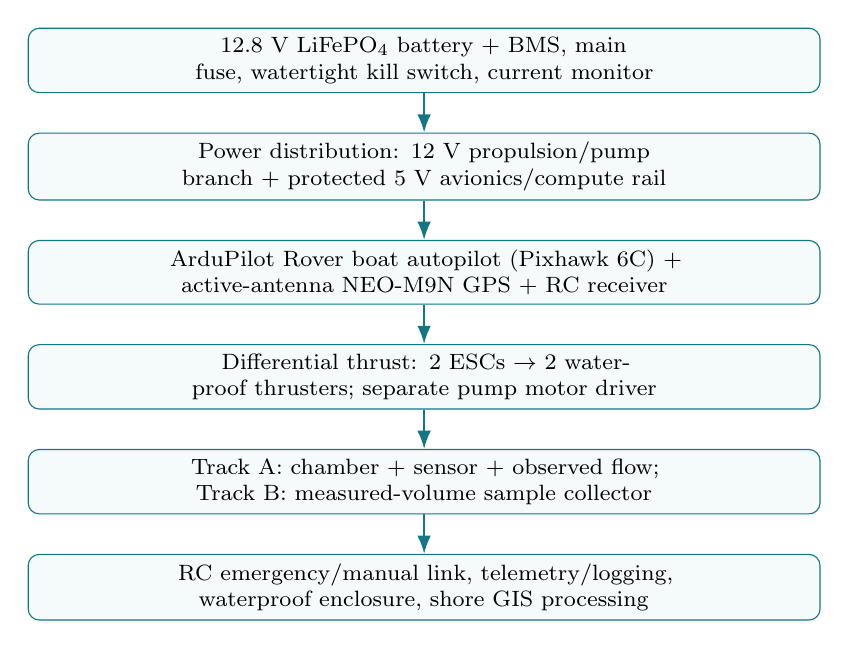
\begin{tikzpicture}[>=Latex,node distance=5mm,b/.style={draw=teal,rounded corners,fill=cream,align=center,text width=0.81\linewidth,minimum height=8mm,font=\footnotesize},a/.style={-Latex,thick,teal}]
\node[b] (bat){12.8 V LiFePO$_4$ battery + BMS, main fuse, watertight kill switch, current monitor};
\node[b,below=of bat] (pdb){Power distribution: 12 V propulsion/pump branch + protected 5 V avionics/compute rail};
\node[b,below=of pdb] (control){ArduPilot Rover boat autopilot (Pixhawk 6C) + active-antenna NEO-M9N GPS + RC receiver};
\node[b,below=of control] (drivers){Differential thrust: 2 ESCs $\rightarrow$ 2 waterproof thrusters; separate pump motor driver};
\node[b,below=of drivers] (sample){Track A: chamber + sensor + observed flow; Track B: measured-volume sample collector};
\node[b,below=of sample] (link){RC emergency/manual link, telemetry/logging, waterproof enclosure, shore GIS processing};
\foreach \u/\v in {bat/pdb,pdb/control,control/drivers,drivers/sample,sample/link} \draw[a] (\u)--(\v);
\end{tikzpicture}
\caption{Block diagram (logical, not complete wiring schematic). RC safety and boat-side logs must not depend on the data-telemetry link.}\end{figure}
\begin{table}[H]\centering\scriptsize
\caption{Prototype system purchase priorities; masses are budget allowances unless specified by manufacturers.}
\begin{tabularx}{\linewidth}{@{}L{2.3cm}L{3.1cm}Y@{}}\toprule
Critical system & Candidate hardware & Procurement/check before commitment\\\midrule
Hull/buoyancy & 2 sealed cylindrical pontoons, $0.90$ m long $\times0.20$ m OD, rigid platform & Measure true sealed displacement, frame strength and wet load\\
Propulsion & 2 Blue Robotics T200 + bidirectional ESCs & 12 V compatible, guards, differential steering and sufficient BMS peak current \cite{T200}\\
Autopilot & Holybro Pixhawk 6C, ArduPilot Rover firmware & Supported hardware; boat mode uses \texttt{FRAME\_CLASS=2} \cite{Pixhawk6C,ArduBoat}\\
RC link & RadioMaster Pocket 2.4 GHz ELRS with matched serial receiver & Manually test kill/hold/failsafe; ensure regional radio compliance \cite{RadioMaster}\\
Telemetry & 2.4 GHz Wi-Fi for near-bank test; optional compatible SiK pair & MAVLink/logs and onboard SD backup, independent of RC \cite{SiK}\\
GNSS & u-blox \textbf{NEO-M9N-00B} module + compatible powered active L1 antenna/compass unit & Verify receiver board has antenna bias circuitry, magnetometer and correct autopilot cable \cite{M9N,SparkM9N}\\
Sampling & SEAFLO 21-Series 12 V diaphragm pump + calibrated flowmeter & 1.2 GPM nameplate is open flow; flow through filters may be lower \cite{Seaflo21}\\
Power & 12.8 V 20 Ah LiFePO$_4$, integrated BMS, LiFePO$_4$ charger & Peak current and fuse coordination; avoid powering motor from flight-controller rail \cite{Bioenno,PM02D}\\
Safety & Sealed electronics, buoyant tether/recovery aid, prop guards, water-leak detector & Safety switch, loss-of-RC configuration, emergency hand retrieval\\\bottomrule\end{tabularx}\end{table}

\section{Radio transmission: RC control versus basic telemetry}
\begin{table}[H]\centering\footnotesize
\caption{Two distinct links; ranges depend on water-level antenna placement and site conditions.}
\begin{tabularx}{\linewidth}{@{}L{2.7cm}L{3.1cm}Y@{}}\toprule
Function & Example & Design consequence\\\midrule
Manual RC override & RadioMaster Pocket, ExpressLRS 2.4 GHz receiver; CRSF serial input & Priority for emergency stop/hold/manual steering; independently test receiver loss, binding and channel assignment \cite{RadioMaster}\\
Basic data transmission & Short-range 2.4 GHz Wi-Fi to shore, or paired SiK MAVLink radio & Send time/GPS/battery/QC/concentration updates; do not stream high-resolution raw video unless capacity verified \cite{SiK}\\
Onboard resilience & SD logging in autopilot or companion computer & Store raw sensor files and logs even when telemetry is lost\\
Frequency compliance & Malaysia MCMC Class Assignment No. 2 of 2025 & Confirm permitted band, module approvals and transmit power before using 433/868/915 MHz \cite{MCMC}\\\bottomrule\end{tabularx}\end{table}
\textbf{Proposed telemetry packet (not a standard specification):} mission ID, timestamp, latitude, longitude, fix quality, battery V/A, motor duty, flow rate, sample ID, counted events, confidence and fault bits. At one compact packet per second, average data rate should be small; verify actual payload and overhead. Record all high-bandwidth images locally.

\section{Autopilot versus in-house control board}
\begin{table}[H]\centering\footnotesize
\caption{Drone flight controller reuse is supported, but a generic drone ECU is not automatically boat-ready.}
\begin{tabularx}{\linewidth}{@{}L{3.0cm}YY@{}}\toprule
Criterion & Pixhawk 6C / ArduPilot Rover & In-house ESP32 / STM32 MCU\\\midrule
Boat software & Official boat variant uses \texttt{FRAME\_CLASS=2}; Rover supports GPS waypoints, Auto, Guided, RTL and Loiter \cite{ArduBoat} & Must implement navigation, steering loops, state estimation and failsafes\\
Hardware & STM32H743, multiple PWM, serial/CAN/GPS interfaces; supported ArduPilot releases \cite{Pixhawk6C,PixhawkFirmware} & Low-cost and flexible I/O, but architecture is student-developed\\
Twin-motor drive & Servo-output differential thrust configuration supported with correct vehicle setup & Two ESC PWM signals; differential thrust and mixing coded manually\\
Mission risk & Mature navigation stack; test firmware, prop guards and mode switching & More coding and test burden, higher risk under two-hour deadline\\
Recommended division & Safety navigation, waypoint execution and RC override & Sampling scheduler, sensor data, flowmeter and CSV telemetry\\\bottomrule\end{tabularx}\end{table}
The supplied \href{https://www.instructables.com/Building-a-Self-Driving-Boat-ArduPilot-Rover/}{self-driving boat tutorial} is a useful build example, but \emph{the governing technical confirmation is ArduPilot's official boat configuration documentation}. Parameter/firmware compatibility must be checked on the chosen board. Set motor outputs, steering and failsafes on the actual boat, not by copying an aircraft mixer.

\section{GPS: active antenna, receiver model and mapping implications}
Specify the \textbf{NEO-M9N-00B} multiconstellation receiver (or Holybro M9N GPS/compass kit with verified module revision). A breakout with \emph{active-antenna bias} is required if using a powered L1 GNSS patch; a bare antenna connector does not guarantee power to an active antenna. u-blox documents support for active antennas, and SparkFun offers NEO-M9N breakouts with external antenna connectors \cite{M9N,SparkM9N}. Representative manufacturer positioning accuracy is roughly $1.5$ m horizontal CEP under specified conditions \cite{M9N}. This is substantial relative to proposed 5 m grid spacing; repeat ground-point checks, keep GNSS well above the waterline, separate from motors, and log actual fix quality. If sub-metre mapping is essential, upgrade to an RTK-capable \emph{different} receiver and surveyed reference corrections rather than claiming the NEO-M9N provides RTK.

\section{Motor comparison: thrust is not hull payload capacity}
An electric thruster's static thrust (kgf) balances \emph{horizontal drag}, not the vertical weight that the hull must float. The allowable carried mass is governed primarily by sealed displacement and stability. Therefore the table compares \textbf{manufacturer thrust and full-throttle electrical load}; it cannot supply a legitimate ``maximum payload kg'' without hull geometry, drag and target speed.
\begin{table}[H]\centering\scriptsize
\caption{Manufacturer-rated propulsion comparison. Full-throttle figures must not be interpreted as average cruise consumption.}
\begin{tabularx}{\linewidth}{@{}L{2.4cm}L{2.25cm}L{2.2cm}L{1.85cm}Y@{}}\toprule
Motor option & Full forward thrust & Full-load electrical at stated V & Proposed load class* & Implication\\\midrule
2 $\times$ T200 (12 V) \cite{T200} & 3.71 kgf \emph{each} & 17 A, 205 W \emph{each} & Prototype 15--25 kg & Good steering authority, \emph{requires throttle limit and peak-current validation}\\
2 $\times$ T500 (12 V) \cite{T500} & 6.0 kgf \emph{each} & 16.9 A, 202 W \emph{each} & Heavier hulls, $>$25 kg & Larger/heavier, likely overkill for sheltered 20-m survey\\
Minn Kota Endura C2 30 (12 V) \cite{MinnKota} & 30 lbf $\approx13.6$ kgf total & up to 30 A, $\approx360$ W & Larger slow platform & Manual tiller/steering adaptation and weight; no differential drive by default\\\bottomrule\end{tabularx}\end{table}
{\footnotesize *The ``load class'' is a proposed \emph{prototype trial mass}, not a rated motor payload or a verified towing capacity. Select actual motors after tow/drag, current and turning tests.\par}
\textbf{Measured-load test:} add 5-kg ballast steps to the completed hull, measure straight-line speed, DC power, steering response, stopping, and recovery. Record operating powers at e.g. 0.15, 0.25 and 0.40 m/s rather than fabricating a vendor speed--payload curve.

\section{Hydrostatics and expected payload mass}
\subsection{Twin-pontoon displacement sizing}
For two sealed circular cylinders, $L=0.90$ m and $D=0.20$ m:
\[V_{\max}=2\pi(D/2)^2L=0.05655\,\mathrm{m}^3\approx56.55\,\mathrm{L}.\]
In fresh water, theoretical maximum fully submerged displaced water mass is approximately $56.55$ kg. Using no more than \textbf{60\% of that displacement as an initial working buoyancy budget} gives about \textbf{33.93 kg} supporting total vessel and payload. This is not a hull stability certification: caps, leaks, trim, loading location and waves may reduce available margin.
\begin{table}[H]\centering\footnotesize
\caption{Illustrative all-up wet mass budget (\texttt{data/payload\_estimate.csv}); validate every line after procurement.}
\begin{tabularx}{\linewidth}{@{}Y r Y r@{}}\toprule
Item & kg & Item & kg\\\midrule
Two 0.9-m pontoons & 2.30 & Frame and enclosure & 2.30\\
2 T200 + 2 ESCs & 1.15 & Autopilot/GPS/radios & 0.45\\
Pump, tubing, filters & 1.27 & Camera and compute & 0.40\\
12.8 V 20 Ah LiFePO$_4$ & 2.40 & Wiring/fuses/extra sensors & 0.90\\
Empty bottles & 0.80 & Eight litres retained water & 8.00\\
Build contingency & 2.00 & & \\\midrule
\textbf{Total wet mass} & \textbf{22.0} & Working buoyancy budget & \textbf{33.93}\\\bottomrule\end{tabularx}\end{table}
\textbf{Important:} Track B with \emph{16 litres retained} instead of 8 adds another 8 kg, raising the vessel to about \textbf{30.0 kg}. It is still under the 33.93-kg illustrative limit but with poor margin for wave, trim and modelling error. An approach with small bottles, fewer stations or progressive sample unloading is preferable to carrying 16 L simultaneously.

\section{Water-pump selection and operating load}
\begin{table}[H]\centering\scriptsize
\caption{Published pump specifications. Quoted open-flow rates are not actual filtered flow; record true Q under backpressure, intake lift and fouling.}
\begin{tabularx}{\linewidth}{@{}L{2.75cm}L{1.4cm}L{2.0cm}L{1.6cm}Y@{}}\toprule
Model & Supply & Flow rating & Electrical load & Use/risk\\\midrule
Adafruit 1150 peristaltic \cite{Adafruit1150} & 12 V & up to 0.10 L/min & 0.2--0.3 A = 2.4--3.6 W & Low contamination contact; too slow for many 1-L stations\\
SEAFLO 21 SFDP1-012-035-21 \cite{Seaflo21} & 12 V & 1.2 GPM $\approx4.5$ L/min & 4.0 A max $\approx48$ W & Candidate collection pump; intermittent duty; measure real flow at filter\\
SEAFLO 500 GPH bilge SFBP1-G500-01 \cite{SeafloBilge} & 12 V & 500 GPH nominal & 1.6 A nominal; 4 A max & High throughput, low head, not precision metering; needs flowmeter\\
SEAFLO 33-Series SFWP1-030-070-33 \cite{Seaflo33} & 12 V & 3.0 GPM $\approx11.3$ L/min & 18 A max $\approx216$ W & Heavy duty, high current; unnecessary for initial small-scale sampling\\\bottomrule\end{tabularx}\end{table}
\textbf{Chosen design basis:} SEAFLO 21 for Track B filling or a bypass-controlled Track A stream, with \emph{measured} flow $\geq1.5$ L/min for Track B in the timing example. Sensitive microchannels may need a \emph{separate low-flow metering stage}; do not force unfiltered river water through them. An inline flowmeter plus calibration against graduated water volume is compulsory. Provide coarse guard, cleanable strainers and a properly routed overflow/backflush. Some pump-contact materials are polymers: use field/process blanks and assess sample contamination.

\section{Power architecture, management, charging and endurance}
\begin{figure}[H]\centering
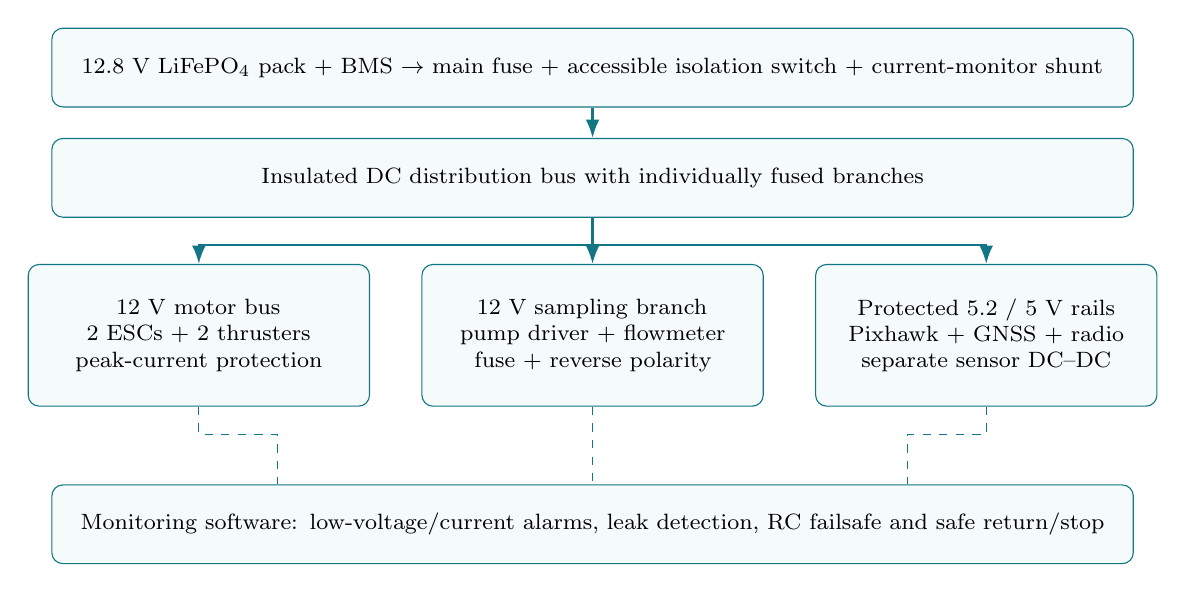
\begin{tikzpicture}[>=Latex,font=\footnotesize,
 bus/.style={draw=teal,rounded corners,fill=cream,text width=13.5cm,minimum height=10mm,align=center},
 branch/.style={draw=teal,rounded corners,fill=cream,text width=4.1cm,minimum height=18mm,align=center},
 arr/.style={-Latex,thick,teal}]
\node[bus] (battery) at (0,0) {12.8 V LiFePO$_4$ pack + BMS $\rightarrow$ main fuse + accessible isolation switch + current-monitor shunt};
\node[bus] (distribution) at (0,-1.4) {Insulated DC distribution bus with individually fused branches};
\node[branch] (motor) at (-5.0,-3.4) {12 V motor bus\\2 ESCs + 2 thrusters\\peak-current protection};
\node[branch] (pump) at (0,-3.4) {12 V sampling branch\\pump driver + flowmeter\\fuse + reverse polarity};
\node[branch] (logic) at (5.0,-3.4) {Protected 5.2 / 5 V rails\\Pixhawk + GNSS + radio\\separate sensor DC--DC};
\node[bus] (safety) at (0,-5.8) {Monitoring software: low-voltage/current alarms, leak detection, RC failsafe and safe return/stop};
\draw[arr](battery)--(distribution);
\foreach \x in {motor,pump,logic} \draw[arr] (distribution.south) -- ++(0,-.35) -| (\x.north);
\draw[dashed,teal] (motor.south) -- ++(0,-.35) -| ([xshift=-4cm]safety.north);
\draw[dashed,teal] (pump.south) -- ++(0,-.35) -| (safety.north);
\draw[dashed,teal] (logic.south) -- ++(0,-.35) -| ([xshift=4cm]safety.north);
\end{tikzpicture}
\caption{Power-distribution concept with genuinely parallel fused motor, pump and logic branches. Dashed paths denote monitoring/fault signalling rather than physical series wiring.}\end{figure}
\textbf{Controller power:} The Holybro PM02D offers regulated 5.2 V up to 3 A from a 2S--12S input, but is \emph{not} a high-current supply for servos, pump or motors \cite{PM02D}. Verify analog/digital module type against the selected Pixhawk connector. Use fused motor and pump circuits; fuses protect wires, not simply the device. \textbf{Battery charging:} A representative Bioenno 12 V 20 Ah LiFePO$_4$ pack includes a protection module with 30 A continuous discharge and specifies a suitable 14.6 V charger (manufacturer example 4 A) \cite{Bioenno}. Do not charge LiFePO$_4$ with an unmatched lead-acid or LiPo charger. Charge in a dry supervised location, disconnected from the boat loads, with supplier-approved charger and appropriate temperature constraints.

\begin{table}[H]\centering\footnotesize
\caption{Averaged survey-power allowances at the DC bus: \emph{engineering assumptions}, not manufacturer measurements.}
\begin{tabularx}{\linewidth}{@{}Yrr@{}}\toprule
Component / combined function & Track A W & Track B W\\\midrule
Two thrusters at low-speed survey (combined) & 50 & 30\\
Autopilot, GNSS, RC receiver & 6 & 6\\
Telemetry / logging & 4 & 2\\
Camera/computer & 9 & 0\\
Pump, \emph{duty-averaged} & 12 & 6\\
Conversion/misc. margin & 7 & 4\\\midrule
\textbf{Estimated average} & \textbf{88} & \textbf{48}\\\bottomrule\end{tabularx}\end{table}
\[E_{\mathrm{nom}}=12.8\times20=256\,\mathrm{Wh},\qquad E_{\mathrm{usable}}=0.80\times256=204.8\,\mathrm{Wh},\qquad t=E_{\mathrm{usable}}/P_{\mathrm{average}}.\]
\begin{table}[H]\centering\footnotesize
\caption{Illustrative 12.8 V, 20 Ah battery operating time: energy-only estimates, ignoring rate/thermal limits and unmodelled loads. Source: \texttt{data/power\_endurance.csv}.}
\begin{tabularx}{\linewidth}{@{}Yrrrr@{}}\toprule
Scenario & Avg W & h & Energy for 2h & 2h energy gate\\\midrule
Track B economical & 48 & 4.27 & 96 Wh & Pass\\
Track A planned & 88 & 2.33 & 176 Wh & Pass (narrow)\\
Track A difficult water & 125 & 1.64 & 250 Wh & Fail\\
High-drive manoeuvres & 180 & 1.14 & 360 Wh & Fail\\
Full-throttle dual T200 at 12 V + loads & 430 & 0.48 & 860 Wh & Fail; BMS also inadequate\\\bottomrule\end{tabularx}\end{table}
\textbf{Critical current warning:} Two T200 thrusters at maximum 12 V load could draw approximately $2\times17=34$ A before other components. The representative Bioenno 20 Ah pack is rated 30 A continuous; full power on both thrusters is therefore \textbf{not permissible} with this battery/BMS. Throttle-limit the ESCs or select a pack with a verified higher discharge rating, suitably rated wires and protection. The $88$ W Track A estimate requires validation with an inline wattmeter on the water, including startup and snagged-propeller cases. \cite{T200,Bioenno}

\section{Time budget and survey choices}
Track A illustrative path: five $20$-m lanes plus four $5$-m lateral moves gives $120$ m. At an assumed $0.25$ m/s the ideal transit is $8$ min. A 60-min effective sensing period plus 25 min setup, turns, recovery, QC and map generation totals $93$ min. A $0.50$-L/min fully interrogated flow yields $30$ L in the sensing period, \emph{not} $30$ L per map cell. Sensor sampling time and intake-delay calibration matter.

Track B illustrative workflow: 16 stations, 1 L per site, effective pumping $1.5$ L/min, $1.2$ min/station for handling and $3$ min/station portable image processing; add 18 min survey movement/setup/mapping. The total is about $95.9$ min. Changing image time to 5 min/site raises it above 120 min. Field concentration and sampling statistics impose a stricter constraint: at around $3.12$ particles/L, a 1-L sample expects only 3.12 particles, equivalent to $57\%$ approximate Poisson standard error \emph{before} sensor losses. The first demonstration should specify a minimum reporting volume and show uncertain/insufficient-count cells rather than inventing a smooth precise heat map.

\section{Risk controls, procurement order and decision}
\begin{enumerate}[leftmargin=*]
\item \textbf{Float test first:} assemble sealed pontoons, weigh all components, add ballast to 22 and 30 kg, check reserve freeboard, trim and wave splash under stationary and moving load.
\item \textbf{Then drive/power test:} two T200 and ESCs (or lower-cost alternative only with measured equivalent performance), current limit and speed tests at full mass. Inspect for overheating and waterproof cable glands.
\item \textbf{Autopilot and RC:} flash appropriate Rover firmware, configure boat class and motor layout, test manual/RTL/Loiter and safe response to link or GNSS loss while tethered.
\item \textbf{Sample circuit:} bench-test the selected pump's \emph{actual} flow through chosen strainers/filter and tubing at target depth; verify sampled volume and cleaning blanks.
\item \textbf{Timing and credibility:} time full 16-sample shoreline chain or Track A effective observed-volume throughput; reject any concept unable to create an auditable map within 120 min.
\item \textbf{Procurement and local radio:} request quotations from university-registered electronics/hardware suppliers, confirm Malaysia radio approval, battery transport/charging and replacement parts.
\end{enumerate}
\textbf{Provisional bill-of-materials decision:} two 0.9-m $\times$ 0.20-m sealed pontoons, two T200 thrusters with compatible reversible ESCs, Pixhawk 6C running ArduPilot Rover boat firmware, external-active-antenna NEO-M9N (GPS/compass integration), ELRS 2.4-GHz RC control, separate low-bandwidth telemetry and local logs, SEAFLO 21 pump plus flowmeter, and 12.8 V 20 Ah LiFePO$_4$ with correct charger and managed current limits. \emph{No full 16-L sample collection without revising the wet-mass, freeboard and storage plan.} The expected 22-kg wet all-up budget is an engineering starting value, not an independently confirmed built boat.

\printbibliography[title={References and manufacturer documentation}]
\end{document}
